\begin{comment}
\chapter*{Annexes}
\addcontentsline{toc}{chapter}{Annexes}
\markboth{Annexes}{}



%Mettez vos annexes ici...

%===================== ANNEXE 1 =====================%
\stepcounter{chapter}
\addtocontents{lot}{\vspace{3.8mm}}
\addtocontents{lof}{\vspace{3.8mm}}



\section*{Annexe 1.~Apprentissage automatique}
\addcontentsline{toc}{section}{Annexe 1.~Apprentissage automatique}


\stepcounter{chapter}
\addtocontents{lot}{\vspace{3.8mm}}
\addtocontents{lof}{\vspace{3.8mm}}

%Mettez vos annexes ici...

%===================== ANNEXE 2 =====================%

\section*{Annexe 2.~H2O.AI}
\addcontentsline{toc}{section}{Annexe 2.~H2O.AI}


H2o.ai est une plate-forme d'apprentissage automatique et d'analyse prédictive open source, en mémoire distribuée, rapide et évolutive qui nous permet de construire des modèles d'apprentissage automatique sur des données volumineuses et de faciliter la production de ces modèles dans un environnement d'entreprise.
H2o.ai nous fournit plusieurs API REST qui a pour but d'échanger des données avec d'autres applications externes. Ci-dessous les différente  étapes  de construction des prédictions (Nous allons s’intéresser aux API REST les plus utilisées)\cite{H2O.AI}.

\textbf {Import du fichier}\\
La première phase c’est l’import d’un fichier d’extension« csv ».
La figure \ref{fig:Importcsv } ci-dessous nous expose les différentes paramètres d'API (import) :
\begin{itemize}
    \item entrée : chemin du fichier à importer;
    \item sortie : le fichier importé.

    \end{itemize} 


          \begin{figure}[htpb]
\centering
    \fcolorbox{black}{white}{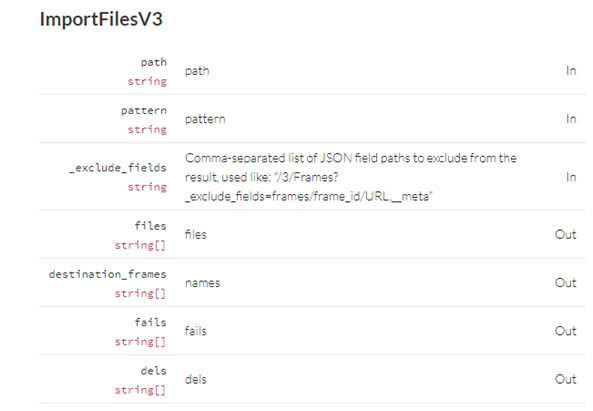
\includegraphics[width=0.9\linewidth]{img/importCsv.png}}
\caption{les paramètres d'import d'un fichier}
\label{fig:Importcsv }
\end{figure}
\newpage
\textbf{H2O FLOW}\\
H2o flow est une interface utilisateur open-source de type carnet de notes pour H2O. Il s'agit d'un environnement interactif basé sur le Web qui vous permet de combiner l'exécution de code, le texte, les mathématiques, les tracés et les médias riches en un seul document \cite{H2OFlow}.\\
La figure \ref{fig:ImportH2oFlow } ci-dessous nous illustre un exemple d'utilisation d'API import avec H2o flow.
          \begin{figure}[htpb]
\centering
    \fcolorbox{black}{white}{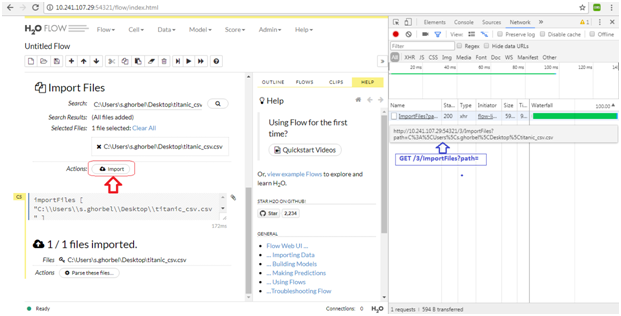
\includegraphics[width=1\linewidth]{img/importH2oFlow.png}}
\caption{Import du fichier avec H2o flow }
\label{fig:ImportH2oFlow }
\end{figure}

%     --------------page2--------%
\newpage
\textbf {Analyse du fichier (ParseSetup en anglais)}\\
Après l’import du fichier, nous devons l'analyser en indiquant en entré son nom.
La figure \ref{fig:ParseSetup } ci-dessous nous expose les différentes paramètres d'API (ParseSetup) :
\begin{itemize}
    \item entrée : nom du fichier à analyser;
    \item sortie : le fichier analysé.

    \end{itemize} 


          \begin{figure}[htpb]
\centering
    \fcolorbox{black}{white}{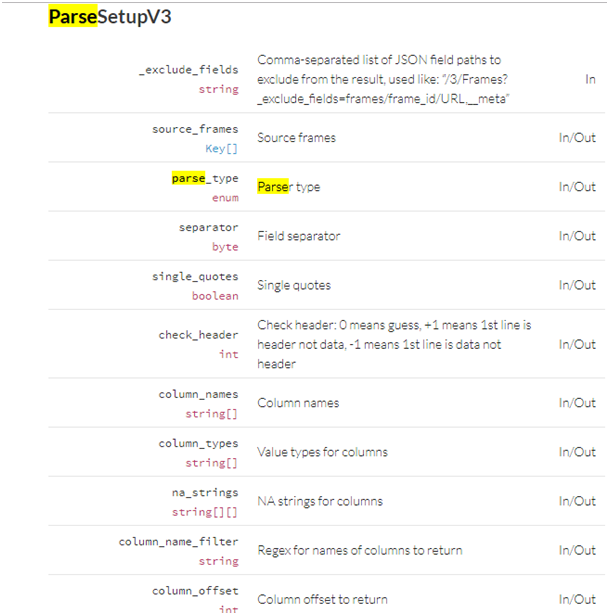
\includegraphics[width=1\linewidth]{img/ParseSetup.png}}
\caption{les paramètres d'analyse d'un fichier}
\label{fig:ParseSetup }
\end{figure}
\newpage
La figure \ref{fig:ParseSetupH2oFlow  } ci-dessous nous illustre un exemple d'utilisation d'API ParseSetup avec H2o flow.
          \begin{figure}[htpb]
\centering
    \fcolorbox{black}{white}{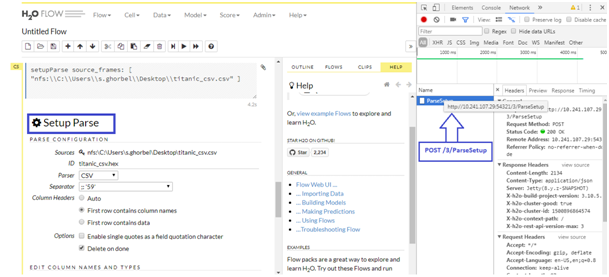
\includegraphics[width=0.9\linewidth]{img/H2oFlowParseSetup.png}}
\caption{Analyse du fichier avec H2o flow }
\label{fig:ParseSetupH2oFlow }
\end{figure}\\
\textbf {Création du modèle}\\
Nous passons maintenant à la phase de la création de modèle en indiquant plusieurs paramètres (données d'apprentissage ,données de test ou validation, variable à prédire, algorithme choisi) comme la montre la figure\ref{fig:BuildModel }.
\begin{figure}[htpb]
\centering
 \fcolorbox{black}{white}{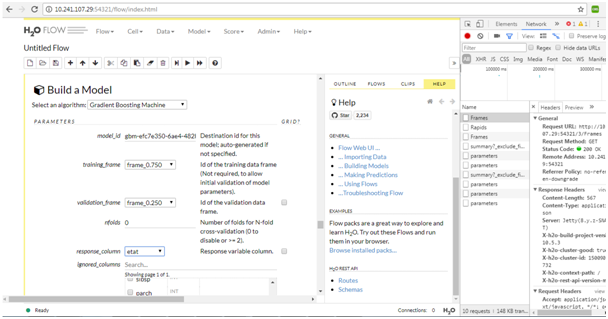
\includegraphics[width=0.9\linewidth]{img/BuildModel.png}}
\caption{Construction du modèle avec H2o flow }
\label{fig:BuildModel }
\end{figure}
\newpage

\textbf {Prédiction}\\
Après avoir construit notre modèle, Nous pourrons effectuer des prédictions, en mentionnant en entrée le modèle et le nom de fichier comme indiqué sur la figure \ref{fig:PredictionH2o } ci-dessous.
\begin{figure}[htpb]
\centering
 \fcolorbox{black}{white}{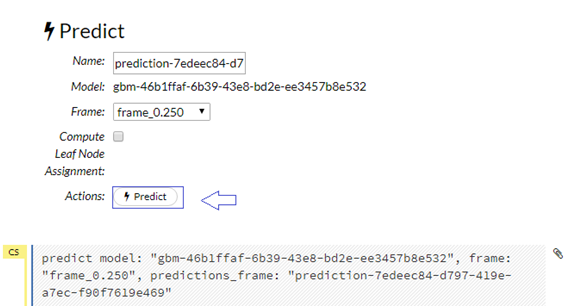
\includegraphics[width=0.75\linewidth]{img/Prediction.png}}
\caption{Prédiction avec H2o flow }
\label{fig:PredictionH2o }
\end{figure}

\textbf {Visualisation des prédictions}\\
La dernière phase consiste à visualiser la colonne de prédiction qui est considérée comme l'étape la plus pertinente dans notre projet comme la montre la figure ci-après.
\begin{figure}[htpb]
\centering
 \fcolorbox{black}{white}{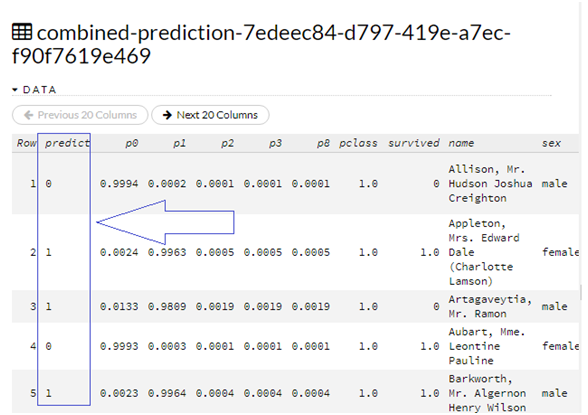
\includegraphics[width=0.75\linewidth]{img/ViewPrediction.png}}
\caption{Visualisation des prédictions avec H2o flow}
\label{fig:ViewData }
\end{figure}

\newpage


%Mettez vos annexes ici...

%===================== ANNEXE 3 =====================%
\stepcounter{chapter}
\addtocontents{lot}{\vspace{3.8mm}}
\addtocontents{lof}{\vspace{3.8mm}}



\section*{Annexe 3.~TENSORFLOW}
\addcontentsline{toc}{section}{Annexe 3.~TENSORFLOW}

\end{comment}